\section{Auswertung}
\label{sec:Auswertung}

\subsection{Die Gitterkonstante $g$}

Wie in Kapitel %\ref{sec:durchfuehrung}
 beschrieben ist bei diesem Versuchsaufbau ein Reflexionsgitter für die Beugung des Lichtes verantwortlich. Für die weitere Auswertung wird daher die Gitterkonstante $g$ benötigt. Das Spektrum einer Quecksilberdampflampe wird untersucht. In Tabelle % \ref{tab:1}
 sind die Winkel aufgetragen, unter denen die verschiedenen Spektrallinien gebeugt werden. Alle Winkel sind relativ zur Position des nullten Maximums bei $\varphi_0=323,6\,\si\degree$ gemessen, sodass dieser Wert von den Winkeln subtrahiert werden muss. Hinzu kommt, dass einlaufender und reflektierter Strahl anders als beim Transmissionsgitter einen Winkel von $2\beta=90\,\si\degree$ einschließen.Daher müssen die Winkel erneut korrigert und $\beta$ abgezogen werden. Dargestellt wird der geometrische Zusammenhang in Abbildung XY DIE FEHLT.
Um die Gitterkonstante $g$ zu bestimmen wird $\sin{\beta}+\sin{\varphi}$ in Abhängigkeit von der Wellenlänge aufgetragen. Die Formel kann aus Abbildung XY und gleichung $\sin{\varphi}=k\lambda/g$ abgeleitet werden. 
\begin{equation}
\sin{\beta}+\sin{\varphi}=\frac{\lambda}{g}
\end{equation}
Daraus ergibt sich mit linearer Regression die Geradengleichung
\begin{equation}
f= \underbrace{(0.001192 \pm 0.000006)\,\frac{1}{\si{\nano\meter}}}_{Steigung\,\triangleq\,\sfrac{1}{g}}x-(0.002 \pm 0.003)
\label{eq:lin_reg}
\end{equation}
mit der reziproken Steigung als Gitterkonstante.
\begin{equation}
g=(839 \pm 3)\,\si{\nano\meter}
\label{eq:gitterkonst}
\end{equation}

\begin{figure}
	\centering
	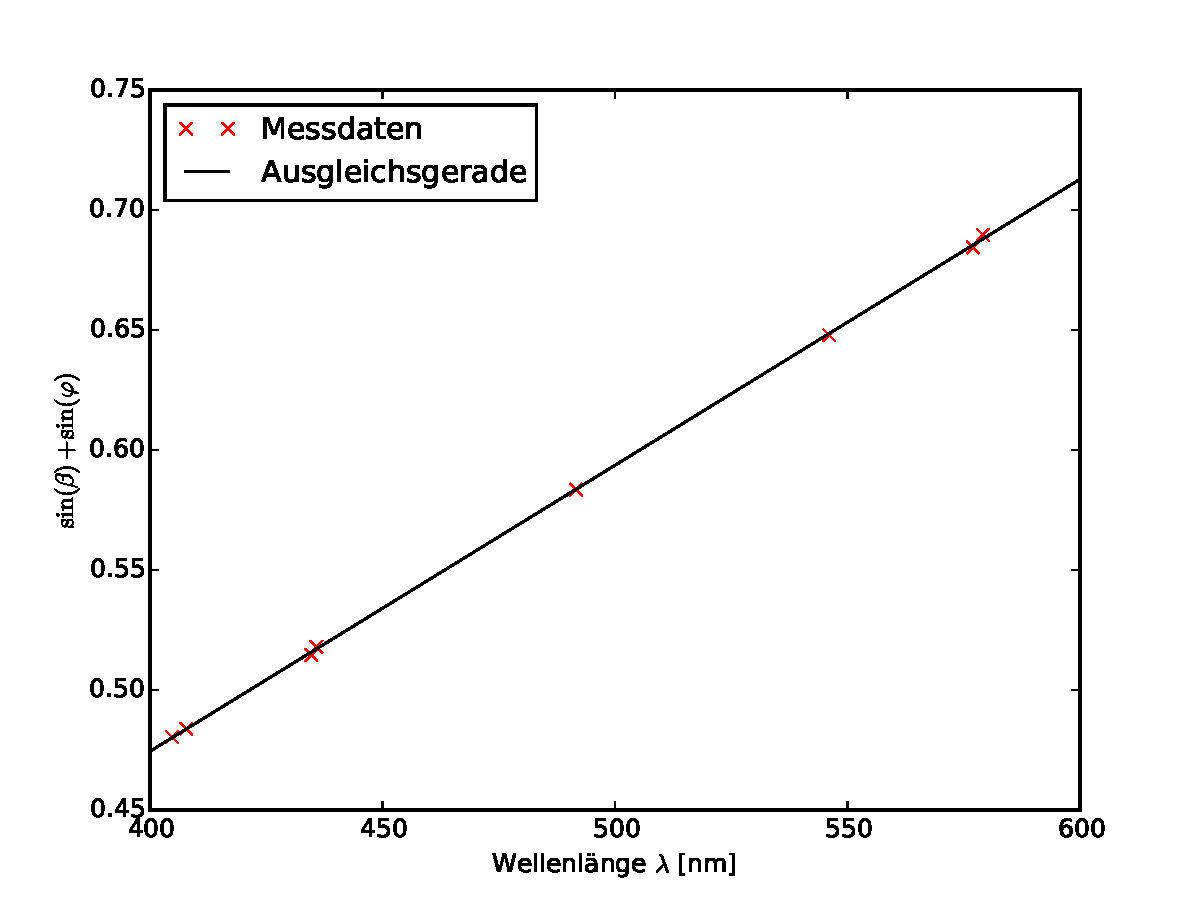
\includegraphics[width=\textwidth]{Bilder/Gitterkonstante.pdf}
	\caption{Ladungen $q$ der Tröpfchen aufgetragen gegen den Radius $r$.}
	\label{fig:gitterkonst}
\end{figure}


\subsection{Untersuchung der Alkalispektren}

Es werden die Sprektren einer Natrium-\footnote{\Bat}, Kalium - und Rubidiumdampflampe ausgemessen. Näher betrachtet werden dabei die Dublett-Linien. Da diese sehr nahe beieinanderliegen wird zur Abstandsmessung ein Okularmikrometer benutzt. Dieses wird zuvor geeicht, wobei $143$ Skalenteile einer Winkeländerung von $\SI{0,3}{\degree}$ entsprechen. Damit kann der Eichfaktor zu $\gamma=0.015\,\si{\nano\meter}\,/Skt.$ berechnet werden. 

In Tabelle NICHT EXISTENT werden die aufgenommenen, sowie um $\varphi_0$ und $\beta$ korrigierten Wete gelistet. Der Winkel, unter welchem die Liniendubletts zu sehen sind, wird durch Mittelwertsbildung der Winkel beider Linien ermittelt.Dabei sind sie um die Strecke $\Delta{s}$ voneinander entfernt. Die Wellenlänge $\lambda$, sowie der Wellenlängenunterschied $\Delta{\lambda}$ werden nach THEORIE berechnet. Mit Gleichung BÖLAA kann nun die Energiedifferenz und damit die Abschirmungszahl bestimmt werden.

Die Dubletts entstehen durch aufspalten des 3P-Niveaus (Na), 4P-Niveaus (Ka) und 5P-Niveaus (Rb).

Damit ergeben sich so Abschirmungszahlen.

Die Abschirmungszahlen ergeben sich mit den Werten aus Tabelle IJWN zu 
\begin{align}
\sigma_\mathup{Na}&=\SI{8.424285(3)}{} \\
\sigma_\mathup{K\:}&=\SI{12.988059(5)}{}\\
\sigma_\mathup{Rb}&=\SI{26.8692(2)}{}
\end{align}
